\section{Introduction}
In this lab course, we work with simulated data from the Belle II 
experiment to develop a fast and efficient simulation pipeline.
The goal is to train and compare machine learning models that can predict 
early in the simulation chain whether an event is likely to survive 
later selection stages. 
This allows us to discard unimportant background events early,
saving computational resources typically spent on full detector simulation 
and reconstruction (processess which are far more comptutaionaly expensive). 
The strategy is illustrated in Fig.~\ref{fig:smart_sim}, 
where a neural network acts as a pre-filter to speed up 
the overall simulation process.
\begin{figure}[h]
    \centering
    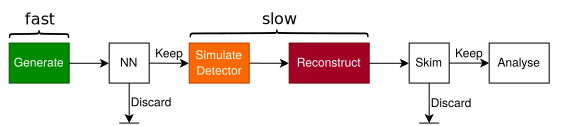
\includegraphics[width=\textwidth]{chapters/introduction/MC_data_flow-keep-discard_NN.png}
\caption{Smart simulation strategy: a neural network filters generated events 
before expensive detector simulation. 
Figure adapted from the official LMU AI Lab repository~\cite{ai-lab-repo}.}
    \label{fig:smart_sim}
\end{figure}
